% Appendix A

\chapter{Figures} % Main appendix title

\label{Figures} % For referencing this appendix elsewhere, use \ref{AppendixA}

\begin{figure}[th]
\centering
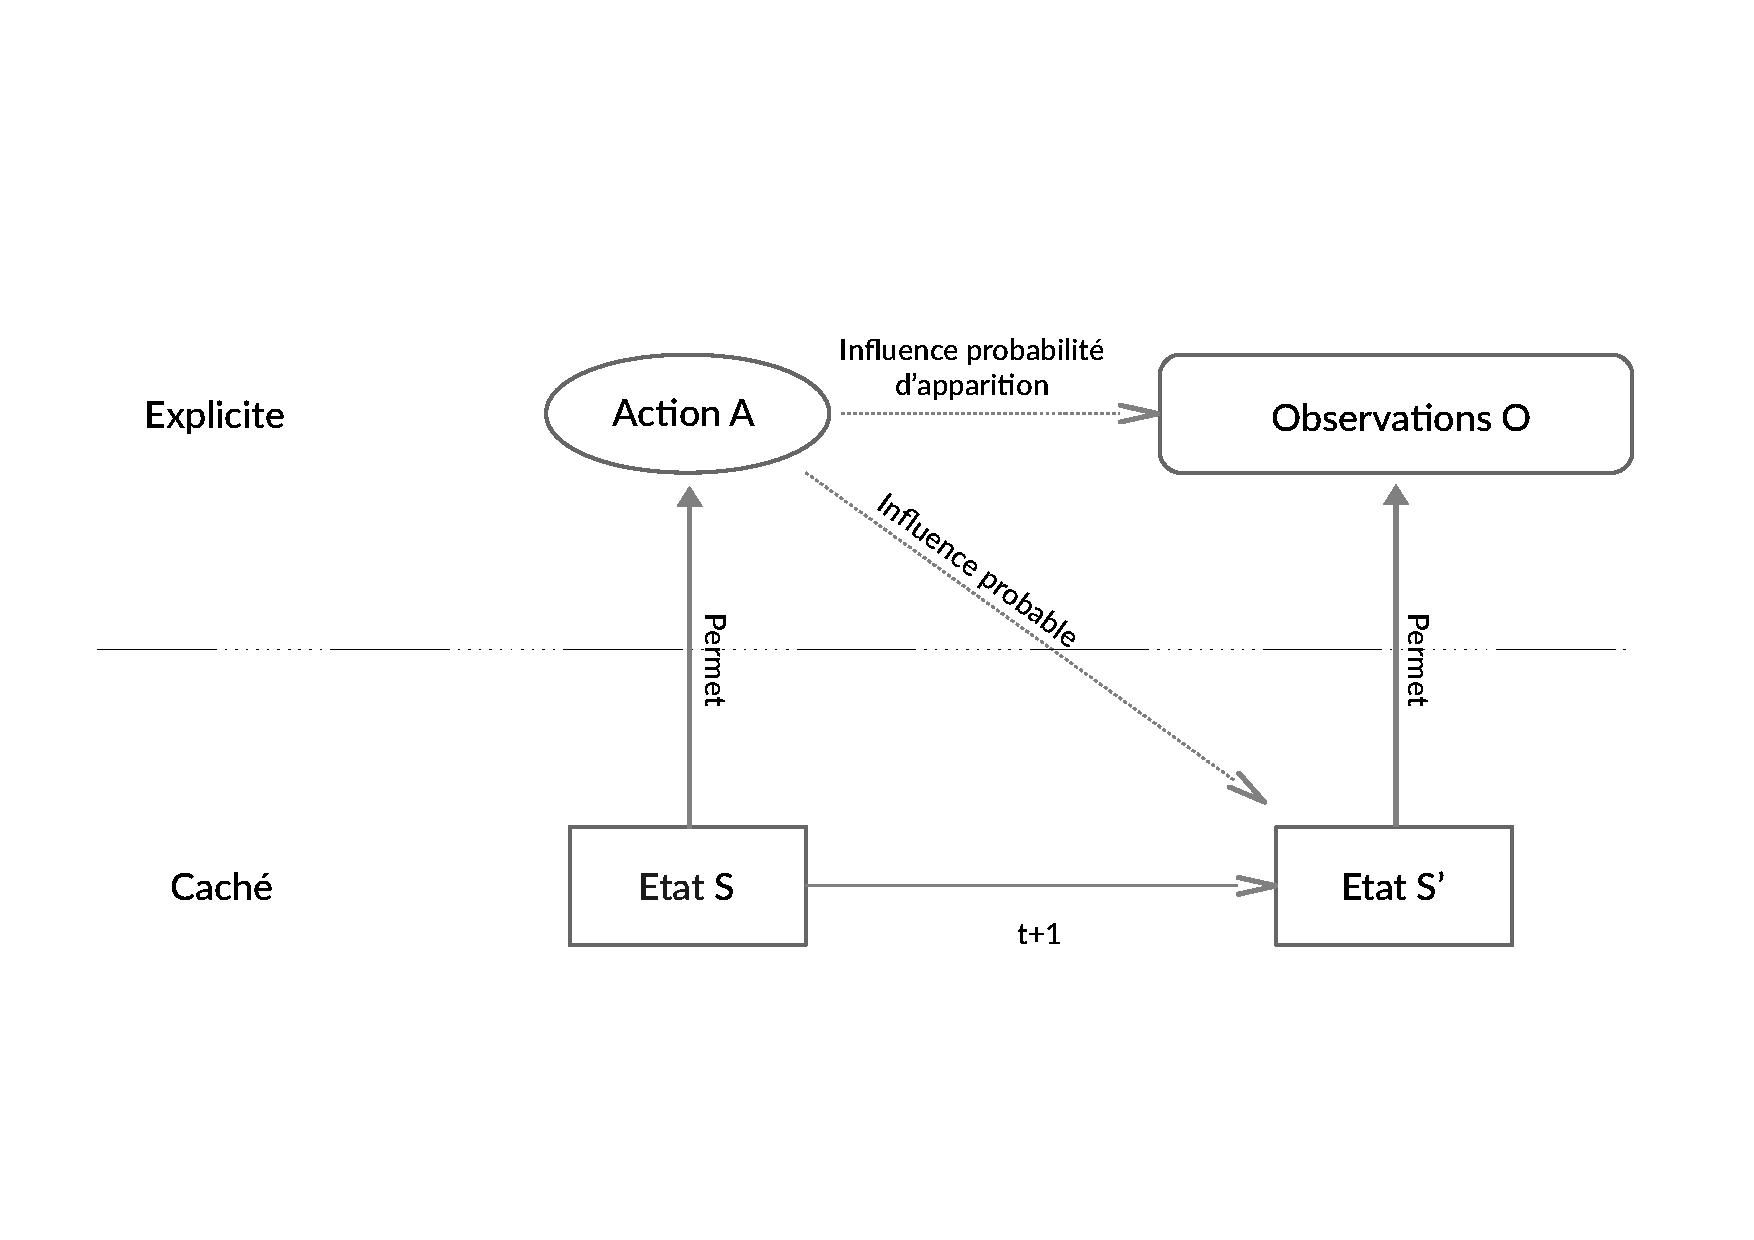
\includegraphics[scale=0.45]{Figures/POMDP}
\decoRule %puts an aesthetic horizontal line below the image
\caption[Figure]{Schéma des interations entre l'agent et son environnement au cours du temps dans un modèle POMDP}
\label{fig:POMDP}
\end{figure}

\begin{figure}[th]
\centering
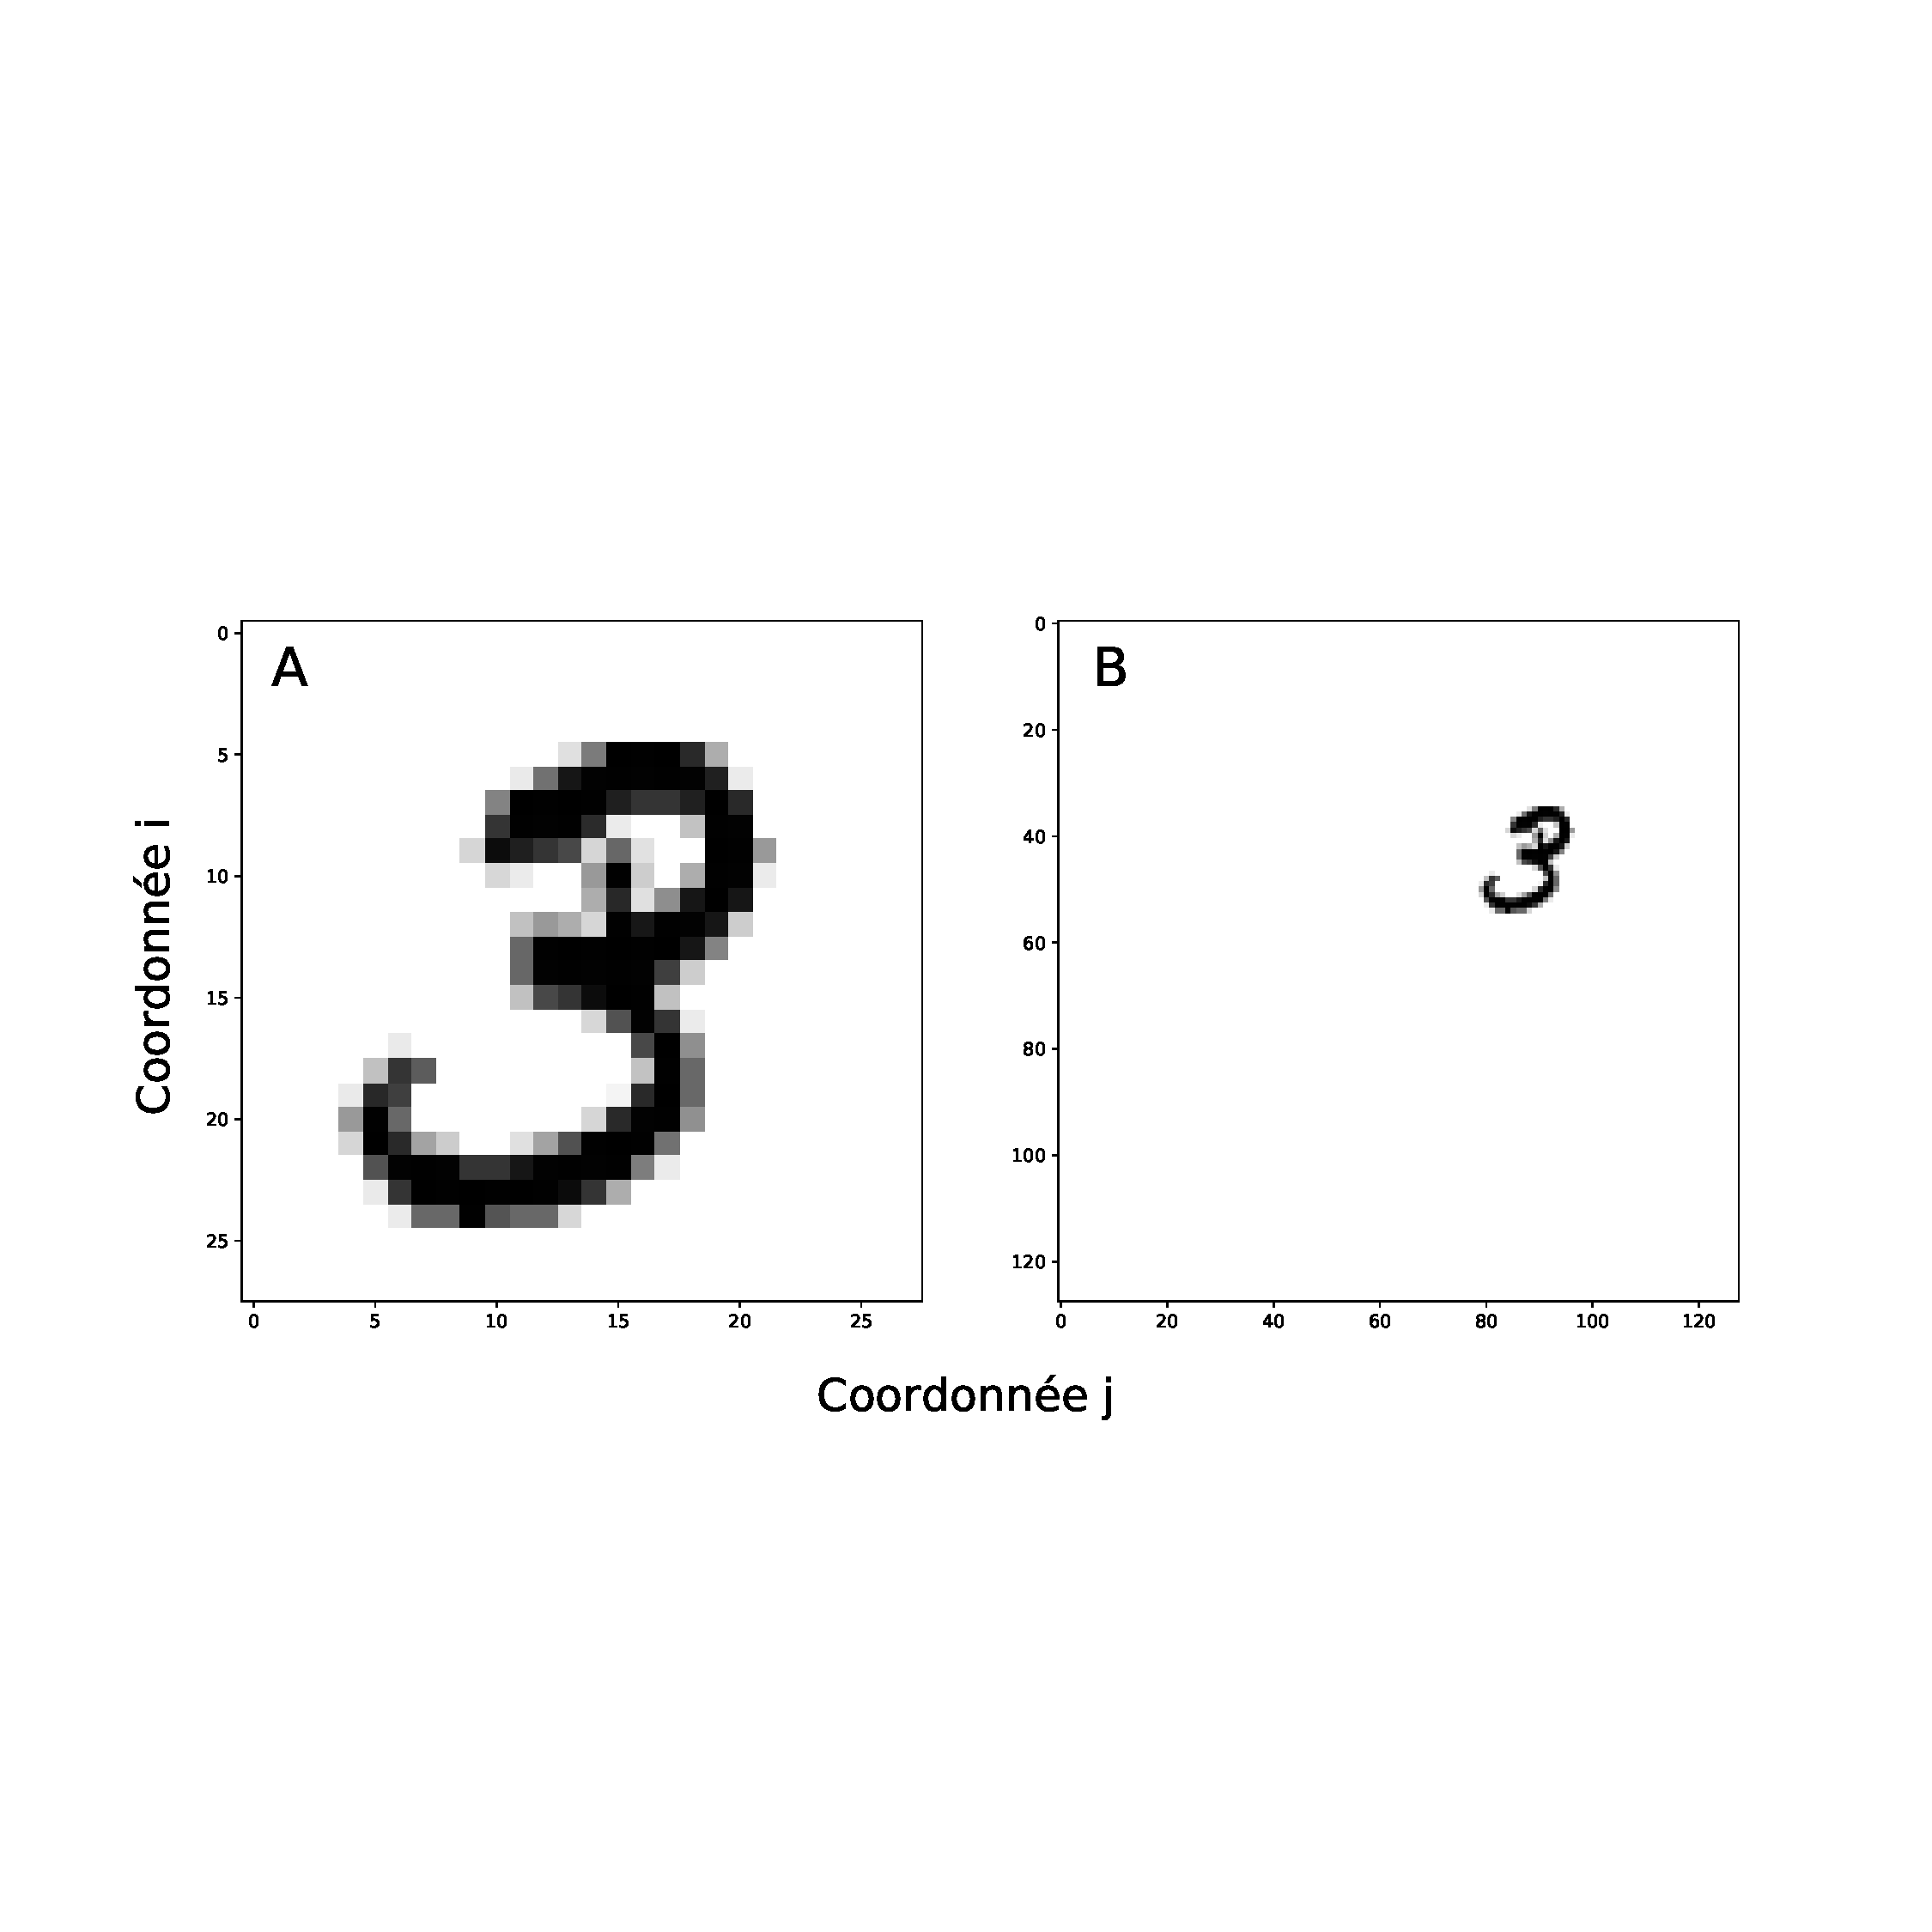
\includegraphics[scale=0.3]{Figures/mnist_reshape}
\decoRule %puts an aesthetic horizontal line below the image
\caption[Figure]{\textbf{A.} Image originale tirée de MNIST ; \textbf{B.} Image après transformation géométrique et placé aux coordonnées $(i=-20,j=25)$}
\label{fig:mnist_reshape}
\end{figure}

\begin{figure}[th]
\centering
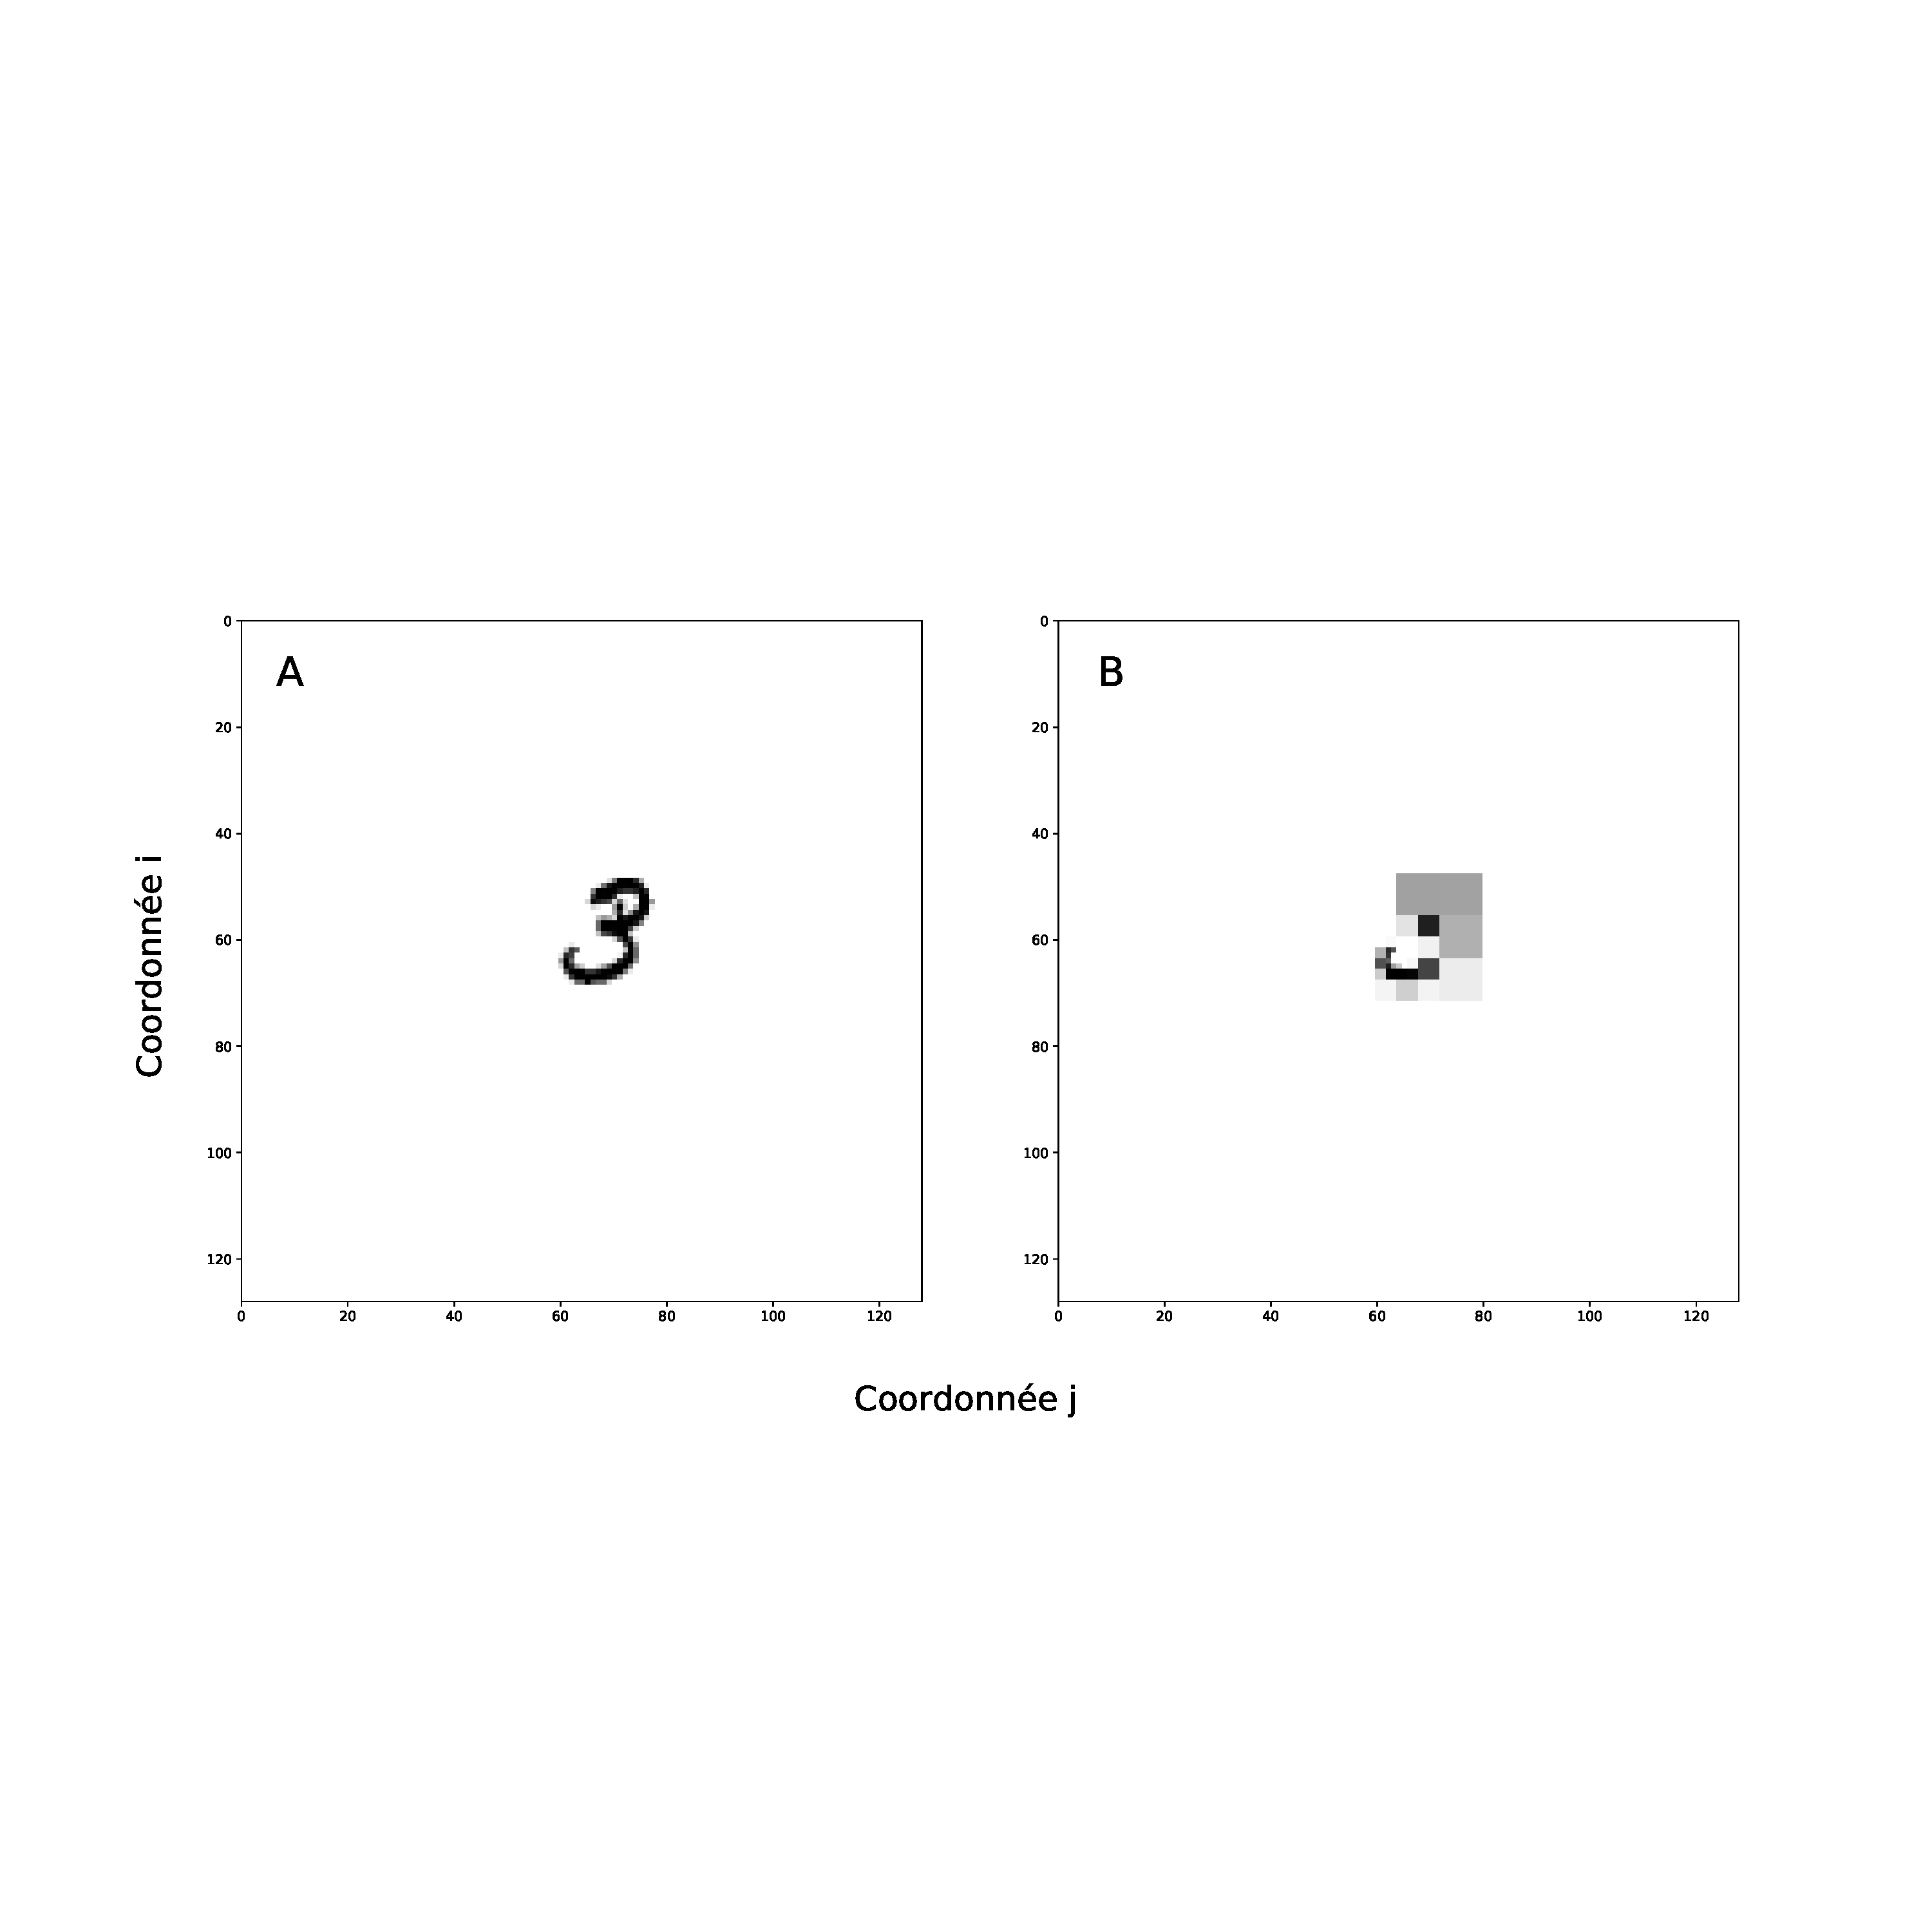
\includegraphics[scale=0.3]{Figures/wavelet_effect}
\decoRule %puts an aesthetic horizontal line below the image
\caption[Figure]{\textbf{A.} Image avant application d'un filtre et placé aux coordonnées $(i=-6,j=6)$ ; \textbf{B.} Image après transformation par vaguelettes (\textit{filtre Wavelets})}
\label{fig:wavelet_effect}
\end{figure}

